\documentclass{beamer}

\usepackage[english]{babel}
\usepackage[utf8]{inputenc}
\usepackage{listings}
\usepackage{datetime}
\usepackage{graphics}
\usepackage{fancybox}
\usepackage{color}
\usepackage{courier}
\usepackage[normalem]{ulem}
\usepackage{tikz}
\usetikzlibrary{shapes,arrows,positioning}
\usetheme{CambridgeUS}
\usecolortheme{seagull}
% Changing of bullet foreground color not possible if {itemize item}[ball]
\DefineNamedColor{named}{Purple}{cmyk}{0.52,0.97,0,0.55}
\setbeamertemplate{itemize item}[triangle]
\setbeamercolor{title}{fg=Purple}
\setbeamercolor{frametitle}{fg=Purple}
\setbeamercolor{itemize item}{fg=Purple}
\setbeamercolor{section number projected}{bg=Purple,fg=white}
\setbeamercolor{subsection number projected}{bg=Purple}

\renewcommand{\dateseparator}{.}
\newcommand{\todayiso}{\twodigit\day \dateseparator \twodigit\month \dateseparator \the\year}
\newcommand{\shell}[1]{\texttt{\small #1}}

\title{Osnove korištenja operacijskog sustava Linux}
\subtitle{02. Rad s datotekama i direktorijima}
\author[Goran Cetušić]{Goran Cetušić\\{\small Nositelj: dr. sc. Stjepan Groš}}
\institute[FER]{Sveučilište u Zagrebu \\
				Fakultet elektrotehnike i računarstva}
				
\date{\todayiso}

\begin{document}
\setbeamertemplate{headline}[]
\setbeamertemplate{footline}{}

\begin{frame}
\maketitle
\end{frame}

\begin{frame}
\frametitle{Sadržaj}
\tableofcontents
\end{frame}

\section{Prikaz sadržaja direktorija}
\begin{frame}[t]
\frametitle{Prikaz sadržaja direktorija}
\begin{itemize}
  \item Naredba \texttt {ls} (engl. \emph{list})
  \begin{itemize}
    \item Prva akcija nakon pokretanja ljuske na nepoznatom sustavu
    \item bez parametara: popis svih datoteka i direktorija, poredan
          abecednim redom, odozgo prema dolje te s lijeva na desno
  \end{itemize}
  \item \textbf {Linux razlikuje velika i mala slova}
  \item Zadatak: pokrenite naredbu \texttt{ls}
\end{itemize}
\end{frame}

\section{Naredbe}
\begin{frame}[t]
\frametitle{Naredbe (1)}
\begin{itemize}
  \item Naredbe se pokreću na sljedeći način
  \begin{itemize}
    \item[] \textless naredba\textgreater \textless opcije\textgreater 
          \textless arugmenti\textgreater
  \end{itemize}
  \item Argumenti označavaju nad čime se vrši naredba
  \begin{itemize}
    \item Često datoteke
    \item Ponekad nisu potrebni
    \begin{itemize}
      \item Primjer \texttt{ls}
    \end{itemize}
    \item Sve piše u man stranicama
  \end{itemize}
\end{itemize}
\end{frame}

\begin{frame}[t]
\frametitle{Naredbe (2)}
\begin{itemize}
  \item Opcije utječu na ponašanje naredbe
  \begin{itemize}
    \item duge opcije (engl. \emph{long options}) počinju s ``-{}-''  
    \item kratke opcije (engl. \emph{short options}) počinju s ``-''
  \end{itemize}
  \item Naredbe obično imaju različite opcije za isto ponašanje
  \begin{itemize}
    \item Primjer: \texttt{man -k regex} \textbf{ili}
          \texttt{man --apropos regex}
  \end{itemize}
  \item Duge opcije su često opisne zbog lakšeg razumijevanja
\end{itemize}
\end{frame}

%\section{Naredba \texttt{ls}}
\begin{frame}[t]
\frametitle{Naredba \texttt{ls} (1)}
\begin{itemize}
  \item Naredba \texttt{ls} prihvaća niz opcija
  \item Često korištena opcije je \texttt{-l} (engl. \emph{long})
  \begin{itemize}
    \item Ispisuje detalje o datotekama i direktorijima
  \end{itemize}
  \item Primjer: Izvršiti sljedeću naredbu
  \item[] \small\texttt{\$ ls -l /bin/sh}
  \item[] \small\texttt{lrwxrwxrwx 1 root root 4 2010-04-29 10:44 /bin/sh 
                        -> bash}
\end{itemize}
\end{frame}

\begin{frame}[t]
\frametitle{Naredba \texttt{ls} (2)}
\begin{itemize}
  \item Stupci kod korištenja \texttt{ls} naredbe s \texttt{-l} opcijom
  \begin{itemize}
    \item Tip datoteke, dozvole, broj referenci, vlasnik, grupa, veličina
          u oktetima, vrijeme zadnje promijene, ime datoteke
  \end{itemize}
  \item Često \texttt{ls} implicitno dodaje opciju \texttt{-{}-color}
  \item Zadatak: Izlistajte direktorij
  \begin{itemize}
    \item[] \texttt{\$ ls -l -{}-color=never}
  \end{itemize}
  \item Usporedite s ispisom bez opcije \texttt{-{}-color}
\end{itemize}
\end{frame}

\begin{frame}[t]
\frametitle{Naredba \texttt{ls} (3)}
\begin{itemize}
  \item Naredbi \texttt{ls} moguće je zadati i ime datoteke/direktorija
  \begin{itemize}
    \item niz odvojen prazninama (označen s \ldots u \texttt{man})
  \end{itemize}
  \item Primjer
  \item[] \small\texttt{\$ ls -l /bin/sh}
  \item[] \small\texttt{lrwxrwxrwx 1 root root 4 2010-04-29 10:44 /bin/sh 
                        -> bash}
  \item Opcija \texttt{-h} (engl. \emph{human readable})
  \begin{itemize}
    \item U kombinaciji s \texttt{-l} ispisuje veličine u čitljivijem
          formatu
  \end{itemize}
\end{itemize}
\end{frame}

\begin{frame}[t]
\frametitle{Naredba \texttt{ls} (4)}
\begin{itemize}
  \item Zadaci
  \begin{itemize}
    \item Izlistajte sadržaj trenutnog direktorija
    \begin{itemize}
      \item Napravite isto korištenjem opcije \texttt{-l}
      \item[] \texttt{\$ ls -l}
      \item Ponovite u kombinaciji s \texttt{-h}
      \item[] \texttt{\$ ls -lh}
    \end{itemize}
    \item Izvršite sljedeće naredbe
    \begin{itemize}
      \item[] \texttt{\$ ls -l /bin/sh}
      \item[] \texttt{\$ ls -l /home}
    \end{itemize}
  \end{itemize}
\end{itemize}
\end{frame}

\section{Skrivene datoteke}
\begin{frame}[t]
\frametitle{Skrivene datoteke}
\begin{itemize}
  \item Na Unix/Linux operacijskom sustavu datoteke čija imena započinju
        točkom su \textbf{skrivene datoteke}
  \begin{itemize}
    \item Ne ispisuju se prilikom izvršavanja naredbe \texttt{ls}, osim
          ako to ne zatražimo
  \end{itemize}
  \item Zadaci
  \begin{itemize}
    \item Isprobati naredbu \texttt{ls} s opcijom \texttt{-a}
    \item Isprobati naredbu \texttt{ls} s opcijama \texttt{-a} i \texttt{-l}
    \item Moguće je kombinirati opcije \texttt{-al} (ili \texttt{-la})
  \end{itemize}
\end{itemize}
\end{frame}

\section{Direktoriji}
\begin{frame}[t]
\frametitle{Direktoriji}
\begin{itemize}
  \item Direktoriji su organizirani kao stablo
  \item U Unix operacijskom sustavu nema diskova
  \begin{itemize}
    \item Sve je \textbf{jedno} stablo direktorija s \textbf{jednim} 
          korijenom
  \end{itemize}
  \centering
  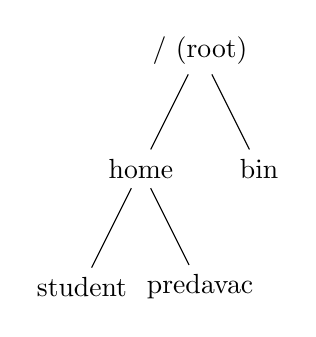
\begin{tikzpicture}
    \node {/ (root)}
        child { 
          node {home} 
          child {node {student} }
          child {node {predavac} }
        }
        child { node {bin} }
    ;
\end{tikzpicture}
\end{itemize}
\end{frame} 


\begin{frame}[t]
\frametitle{Trenutni direktorij}
\begin{itemize}
  \item Trenutni (tekući, radni) direktorij je direktorij u kojem se
        nalazimo
  \begin{itemize}
    \item Korisnik ili aplikacija
  \end{itemize}
  \item Možemo saznati koji je radni direktorij naredbom \texttt{pwd} 
        \\(engl. \emph{print working directory})
  \item Zadatak
  \begin{itemize}
    \item isprobati naredbu \texttt{pwd}
  \end{itemize}
\end{itemize}
\end{frame}

\begin{frame}[t]
\frametitle{Matični direktorij}
\begin{itemize}
  \item Svaki korisnik ima matični (engl. \emph{home}) direktoriji
  \begin{itemize}
    \item Služi za spremanje osobnih podataka i postavki
    \item Korisnik ima ovlasti za pisanje i brisanje unutar svog matičnog
          direktorija
    \item Izvan matičnog direktorija \textbf{nije dozvoljeno} pisanje 
          korisnicima koji nisu administratori
  \end{itemize}
  \item Neposredno nakon pokretanja ljuske, trenutni direktorij je matični
        direktorij 
\end{itemize}
\end{frame}

\begin{frame}[t]
\frametitle{Relativna i apsolutna staza (1)}
\begin{itemize}
  \item Položaj datoteke ili direktorija na Unix/Linux sustavu može se 
        zadati
  \begin{itemize}
    \item Apsolutno - počinje znakom ``\texttt{/}''
    \begin{itemize}
      \item[] Primjer: \texttt{/home/student/okosl}
    \end{itemize}
    \item Relativno 
    \begin{itemize}
      \item[] Primjer: \texttt{student/okosl}
    \end{itemize}
  \end{itemize}

  \item Relativna staza ovisi o trenutnom direktoriju
  \begin{itemize}
    \item Ako ste u direktoriju \shell{/home}, apsolutna staza za
          \textbf{student/okosl} je \textbf{/home/student/okosl}
  \end{itemize}
\end{itemize}
\end{frame}

\begin{frame}[t]
\frametitle{Relativna i apsolutna staza(2)}
\begin{itemize}
  \item Znak ``\texttt{/}'' označava korijenski direktorij
  \begin{itemize}
    \item Kod staze znači da je sljedeći direktorij poddirektorij
          prethodnog
  \end{itemize}
  \centering
  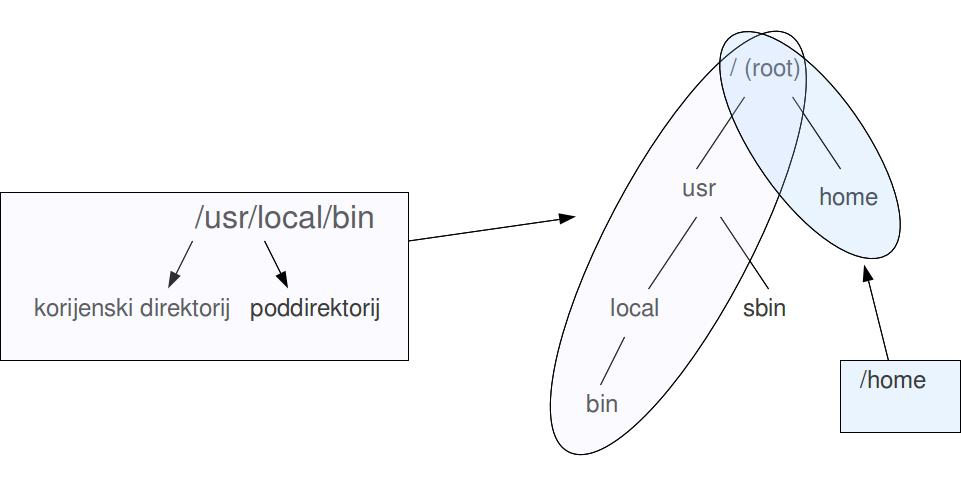
\includegraphics[scale=0.3]{filetree_detail}
%  \begin{tikzpicture}
%    \node { / (root)}
%        child { 
%          node {usr} 
%          child {
%            node {local} 
%            child { node {bin} }
%          }
%          child {node {sbin} }
%        }
%        child { node {home} }
%    ;
%    \end{tikzpicture}
\end{itemize}
\end{frame}

\begin{frame}[t]
\frametitle{Stvaranje direktorija (1)}
\begin{itemize}
  \item Stvaranje novog direktorija obavlja se naredbom \texttt{mkdir}
  \begin{itemize}
    \item Argument je relativno ili apsolutno ime direktorija koji se
          stvara
  \end{itemize}
  \item Zadatak
  \begin{itemize}
    \item Stvoriti direktorije VJEZBA u tekućem direktoriju
    \item Provjeriti naredbom \texttt{ls} podatke o novom direktoriju
    \item Što se dogodi ako naredbi \texttt{ls} kao argument navedemo
          ime direktorija?
  \end{itemize}
\end{itemize}
\end{frame} 

\begin{frame}[t]
\frametitle{Stvaranje direktorija (2)}
\begin{itemize}
  \item Zadatak
  \begin{itemize}
    \item Izvršite naredbu \texttt{mkdir VJEZBA/dir1}
    \item Izlistajte sadržaj direktorija \texttt{VJEZBA}
    \item Izvršite naredbu \texttt{mkdir VJEZBA/dir1/poddir}
    \item Izvršite naredbu \texttt{mkdir VJEZBA/dir2/poddir}
    \item Što se dogodilo u zadnjem slučaju? 
  \end{itemize}
  \item Naredba \texttt{mkdir} prihvaća opciju \texttt{-p}
  \begin{itemize}
    \item Stvara sve potrebne poddirektorije ako ne postoje
  \end{itemize}
\end{itemize}
\end{frame}

\begin{frame}[t]
\frametitle{Stvaranje direktorija (3)}
\begin{itemize}
  \item Zadatak
  \begin{itemize}
    \item Korsteći naredbu \texttt{mkdir} s opcijom \texttt{-p} stvoriti
          hijerarhiju direktorija prikazanih na slici
    \begin{itemize}
      \item[-] \$HOME označava vaš matični direktorij i njega nije
                potrebno stvoriti (tu se trenutno nalazite)
    \end{itemize}
  \end{itemize}
  \centering
  \begin{tikzpicture}
    \node{\$HOME}
      child {
        node {a}
        child { node {1} }
        child { node {2} }
      }
      child {
        node {b}
      }
      child {
        node {c}
        child {
          node {3}
          child { node {f} }
      }
    }
  ;
  \end{tikzpicture}
\end{itemize}
\end{frame}

\begin{frame}[t]
\frametitle{Prikaz sadržaja direktorija}
\begin{itemize}
  \item Naredba \texttt{ls} ispisuje sadržaj direktorija
  \item Zadatak
  \begin{itemize}
    \item Izlistati sadržaj direktorija \texttt{a} naredbom \texttt{ls}
  \end{itemize}
  \item Opcijom \texttt{-d} ne izlistava se sadržaj direktorija već 
        informacije o samom direktoriju
  \item Zadatak
  \begin{itemize}
    \item Izlistati sadržaj direktorija \texttt{a} koristeći opciju 
          \texttt{-d}
  \end{itemize}
\end{itemize}
\end{frame}
    

\begin{frame}[t]
\frametitle{Promjena direktorija (1)}
\begin{itemize}
  \item Promjena direktorija obavlja se naredbom \texttt{cd} (engl. 
        \emph{change directory})
  \item Novi direktorij se zadaje 
  \begin{itemize}
    \item relativno u odnosu na tekući direktorij
    \item apsolutno u odnosu na korijenski direktorij  
  \end{itemize}
  \item Zadatak
  \begin{itemize}
    \item Provjeriti koji je tekući direktorij
    \item Ući u direktorij VJEZBA, vratiti se u prethodni
  \end{itemize}
\end{itemize}
\end{frame}

\begin{frame}[t]
\frametitle{Promjena direktorija (2)}
\begin{itemize}
  \item Rješenje ide otprilike ovako
  \begin{itemize}
    \item[] \texttt{\$ pwd}
    \item[] \texttt{/home/student}
    \item[] \texttt{\$ cd VJEZBA}
    \item[] \texttt{\$ pwd}
    \item[] \texttt{/home/student/VJEZBA}
    \item[] \texttt{\$ cd ..} (ili \texttt{cd /home/student})
    \item[] \texttt{\$ pwd}
    \item[] \texttt{/home/student}
  \end{itemize}
\end{itemize}
\end{frame}
 
\begin{frame}[t]
\frametitle{Promjena direktorija(3)}
\begin{itemize}
  \item Naredba \texttt{cd} bez argumenata vraća u matični direktorij
  \item Zadatak
  \begin{itemize}
    \item Otići u korijenski direktorij (\texttt{/})
    \item Izlistati sadržaj korijenskog direktorija
    \item Vratiti se u matični direktorij
  \end{itemize}
\end{itemize}
\end{frame}

\begin{frame}[t]
\frametitle{Posebni direktoriji (1)}
\begin{itemize}
  \item Svaki direktorij sadrži dva posebna direktorija
  \begin{itemize}
    \item \texttt{..} roditeljski direktorij (engl. \emph{parent directory})
    \item \texttt{.} tekući direktorij (engl. \emph{current directory})
  \end{itemize}
  \item Primjeri
  \begin{itemize}
    \item \texttt{cd . } 
    \begin{itemize}
      \item Mijenja direktorij u tekući direktorij, efektivno nema 
               promjene
    \end{itemize}
    \item \texttt{cd .. }
    \begin{itemize}
      \item Mijenja trenutni direktorij u direktorij iznad
    \end{itemize}
  \end{itemize}
\end{itemize}
\end{frame}

\begin{frame}[t]
\frametitle{Posebni direktoriji (2)}
\begin{itemize}
  \item Koriste se za relativno ``adresiranje'' direktorija
  \item Ne mogu ići van korijenskog direktorija, tj.
  \begin{itemize}
    \item[] \texttt{/../../} je isto što i \texttt{/}
  \end{itemize}
  \item Česta pogreška korisnika DOS-a
  \begin{itemize}
    \item Upisivanje \texttt{cd..} (bez razmaka)
    \item Na Unixu to je posebna naredba (``.'' može biti sastavni dio 
          imena)
  \end{itemize}
\end{itemize}
\end{frame}

\begin{frame}[t]
\frametitle{Posebni direktoriji (3)}
\begin{itemize}
  \item Posebni direktoriji se mogu koristiti u imenima datoteka
  \flushleft
  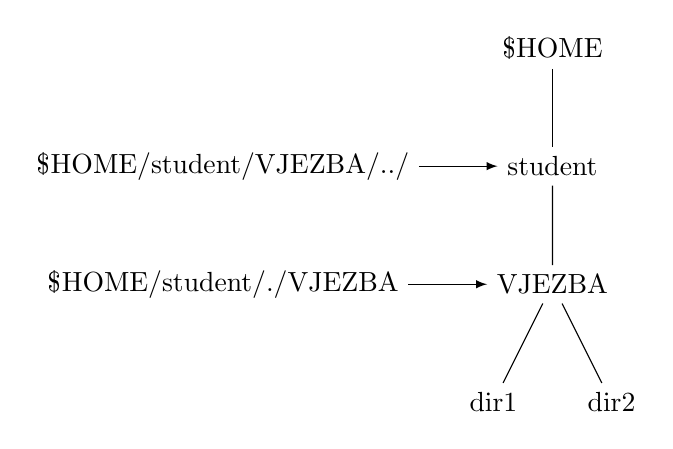
\begin{tikzpicture}[auto, >=latex]
  \node{\$HOME}
    child {
      node (a) {student} 
      child {
        node (b) {VJEZBA}
        child { node {dir1} }
        child { node {dir2} }
      }
    }
  ;
  \node (c) [left=1cm of a] {\$HOME/student/VJEZBA/../}; 
  \node (d) [left=1cm of b] {\$HOME/student/./VJEZBA};
  \draw[->] (c) -- (a);
  \draw[->] (d) -- (b);
  \end{tikzpicture}
\end{itemize}
\end{frame}

\begin{frame}[t]
\frametitle{Posebni direktoriji (4)}
\begin{itemize}
  \item Zadatak
  \begin{itemize}
    \item Provjeriti koji je tekući direktorij i ući u direktorij VJEZBA
    \item Vratiti se u prethodni direktorij korištenjem ..
  \end{itemize}
  \item Zadatak
  \begin{itemize}
    \item Otići u direktorij \texttt{\$HOME/a/2} 
    \item Koristeći relativno adresiranje tekućeg direktorija prebaciti se
          u \texttt{\$HOME/c/3/f}
    \item Vratiti se u matični direktorij
  \end{itemize}
\end{itemize}
\end{frame}

\section{Kopiranje datoteka}
\begin{frame}[t]
\frametitle{Kopiranje datoteka (1)}
\begin{itemize}
  \item Kopiranje se obavlja naredbom \texttt{cp} (engl. \emph{copy})
  \item Sintaksa naredbe 
  \begin{itemize}
    \item \texttt{cp \textless datoteka1\textgreater 
                     \textless datoteka2\textgreater}
    \begin{itemize}
      \item[-] Stvara kopiju datoteke \texttt{datoteka1} i naziva ju 
               \texttt{datoteka2}
    \end{itemize}
    \item \texttt{cp \textless datoteka1\textgreater 
                     \textless datoteka2\textgreater 
                     \textless direktorij\textgreater}
    \begin{itemize}
      \item[-] Kopira datoteke \texttt{datoteka1} i \texttt{datoteka2} u
               direktorij pod nazivom \texttt{direktorij}
    \end{itemize}
  \end{itemize}
  \item Imena datoteka mogu biti apsolutna ili relativna
\end{itemize}
\end{frame}

\begin{frame}[t]
\frametitle{Kopiranje datoteka (2)}
\begin{itemize}
  \item Zadatak
  \begin{itemize}
    \item Pozicionirati se u matični direktorij
    \item Kopirati datoteku \texttt{/bin/vi} u svoj matični direktorij pod
          nazivom \texttt{vi1}
    \item Kopirati datoteku \texttt{vi1} u datoteku pod nazivom 
          \texttt{vi}, također u matičnom direktoriju
    \item Provjeriti da su datoteke ispravno kopirane
  \end{itemize}
\end{itemize}
\end{frame}

%\section{Kopiranje direktorija}
\begin{frame}[t]
\frametitle{Kopiranje direktorija (1)}
\begin{itemize}
  \item Kopiranje direktorija (i svih poddirektorija i datoteka) se 
        obavlja zadavanjem opcije \texttt{-r} naredbi \texttt{cp}
  \begin{itemize}
    \item[] \texttt{cp -r \textless direktorij1\textgreater
                          \textless direktorij2\textgreater}
    \item Ako \texttt{direktorij2} ne postoji, bit će kreiran kao kopija
          prvog
    \item Ako \texttt{direktorij2} postoji, \texttt{direktorij1} će biti
          kopiran u njega 
  \end{itemize}
  \item Oba argumenta mogu biti apsolutna ili relativna
  \item Dosta naredbi ima neku opciju za rekurziju
\end{itemize}
\end{frame}

\begin{frame}[t]
\frametitle{Kopiranje direktorija (2)}
\begin{itemize}
  \item Zadatak
  \begin{itemize}
    \item Pokušati kopirati direktorij \texttt{\$HOME/a/1} u direktorij 
          \texttt{\$HOME/c/3} prvo bez, a potom s opcijom \texttt{-r}
    \item Provjeriti sadržaj odredišnog direktorija
    \item Prijetite kako je nemoguće zamijeniti datoteku s direktorijem
          ako on već postoji
    \begin{itemize}
      \item[-] Rezultirat će kopiranjem datoteke u direktorij
    \end{itemize}
  \end{itemize}
\end{itemize}
\end{frame}

\section{Preimenovanje i premještanje datoteka}
\begin{frame}[t]
\frametitle{Preimenovanje i premještanje datoteka}
\begin{itemize}
  \item Premještanje i preimenovanje se obavlja \textbf{jednom} naredbom
        \texttt{mv} \\(engl. \emph{move})
  \item Sintaksa naredbe 
  \begin{itemize}
    \item[] \texttt{mv \textless datoteka1\textgreater
                       \textless datoteka2\textgreater}
    \begin{itemize}
      \item Mijenja ime datoteke \texttt{datoteka1} u \texttt{datoteka2}
    \end{itemize}
    \item[] \texttt{mv \textless datoteka1\textgreater 
                       \textless datoteka2\textgreater 
                       \textless direktorij\textgreater}
    \begin{itemize}
      \item Premješta datoteke \texttt{datoteka1} i \texttt{datoteka2}
               u direktorij pod nazivom \texttt{direktorij}
    \end{itemize}
  \end{itemize}
\end{itemize}
\end{frame}

\begin{frame}[t]
\frametitle{Preimenovanje i premještanje direktorija}
\begin{itemize}
  \item Naredba \texttt{mv} može služiti za preimenovanje direktorija 
  \begin{itemize}
    \item Sintaksa je ista kao za premještanje datoteka
    \item Može pomicati i direktorije bez potrebe za dodatnim argumentima
  \end{itemize}
  \item Zadatak
  \begin{itemize}
    \item Preimenovati direktorij \texttt{VJEZBA} u \texttt{STARO}
    \item Pomaknuti direktorij \texttt{STARO} u direktorij 
          \texttt{\$HOME/a}
    \begin{itemize}
      \item Provjeriti uspješnost izvršavanja naredbe
    \end{itemize}
  \end{itemize}
\end{itemize}
\end{frame}

\section{Brisanje datoteka i direktorija}
\begin{frame}[t]
\frametitle{Brisanje datoteka}
\begin{itemize}
  \item Brisanje datoteka i direktorija obavlja se naredbom \texttt{rm}
        (engl. \emph{remove})
  \item Sintaksa naredbe
  \begin{itemize}
    \item[] \texttt{rm \textless ime datoteke\textgreater}
  \end{itemize}
  \item Zadatak
  \begin{itemize}
    \item Pokušati obrisati nepostojeću datoteku
    \item Pokušati obrisati direktorij
  \end{itemize}
\end{itemize}
\end{frame}

\begin{frame}[t]
\frametitle{Brisanje direktorija (1)}
\begin{itemize}
  \item Za brisanje direktorija koristi se naredba \texttt{rmdir}
  \begin{itemize}
    \item Direktorij mora biti prazan (osim posebnih direktorija)
  \end{itemize}
  \item Sintaksa
  \begin{itemize}
    \item[] \texttt{rmdir \textless ime direktorija\textgreater}
  \end{itemize}
  \item Zadatak
  \begin{itemize}
    \item Pokušati obrisati direktorij \texttt{\$HOME/b}
    \item Pokušati obrisati direktorij \texttt{\$HOME/a}
  \end{itemize}
\end{itemize}
\end{frame}

\begin{frame}[t]
\frametitle{Brisanje direktorija (2)}
\begin{itemize}
  \item Ako direktorij nije prazan, možemo koristiti naredbu \texttt{rm}
        sa sljedećim opcijama
  \begin{itemize}
    \item \texttt{-r} rekurzivno brisanje
    \item \texttt{-f} prisilno brisanje
  \end{itemize}
  \item Sintaksa je 
  \begin{itemize}
    \item[] \texttt{rm -rf \textless ime direktorija\textgreater\ldots}
  \end{itemize}
  \item[] OPREZNO S TOM NAREDBOM! NEMA POVRATA OBRISANIH PODATAKA!
\end{itemize}
\end{frame}

\begin{frame}[t]
\frametitle{Brisanje direktorija (3)}
\begin{itemize}
  \item Naredba \texttt{rm} je dosta opasna, zato se može koristiti s 
        opcijama \\\texttt{-i} ili \texttt{-I}
  \item Zadatak
  \begin{itemize}
    \item Pozicionirati se u direktorij \texttt{VJEZBA}
    \item Pokušati obrisati direktorij \texttt{VJEZBA}
  \end{itemize}
  \item Zadatak
  \begin{itemize}
    \item Jednom naredbom \texttt{rm} i korištenjem opcije \texttt{-I} 
          obrisati direktorije \texttt{\$HOME/a}, \texttt{\$HOME/b} i 
          \texttt{\$HOME/c}
  \end{itemize}
\end{itemize}
\end{frame}

\section{Nazivi datoteka}
\begin{frame}[t]
\frametitle{Nazivi datoteka (1)}
\begin{itemize}
  \item Linux razlikuje velika i mala slova
  \item Imena datoteka mogu sadržavati sve znakove osim /, koji označava
        poddirektorij
  \item Imena mogu sadržavati praznine
  \begin{itemize}
    \item Praznine obično znače sljedeći argument naredbe 
  \end{itemize}
  \item Primjer:
  \begin{itemize}
    \item[] \texttt{\$ mkdir novi direktorij}
  \end{itemize}
\end{itemize}
\end{frame}

\begin{frame}[t]
\frametitle{Nazivi datoteka (2)}
\begin{itemize}
  \item Datoteka ili direktorij s prazninama označava se se na dva načina 
  \begin{itemize}
    \item Stavljanje imena datoteke pod navodnike
    \item ubacivanje znaka \textbackslash{} (engl. \emph{backslash}) 
          prije svake praznine
  \end{itemize}
  \item Primjer:
  \begin{itemize}
    \item[] Stvoriti i zatim obrisati direktorija \texttt{"nova
            datoteka 2"}
    \item[] \texttt{\$ mkdir "nova datoteka 2"}
    \item[] \texttt{\$ rmdir nova\textbackslash{} datoteka\textbackslash{}
                     2}
  \end{itemize}
\end{itemize}
\end{frame}

\end{document}

